\documentclass[preprint,12pt,authoryear]{elsarticle}

\usepackage[utf8]{inputenc}
\usepackage[T1]{fontenc}
\usepackage{amsmath}
\usepackage{lmodern}
\usepackage{XCharter}
\usepackage[xcharter,vvarbb]{newtxmath}
\usepackage{microtype}
\usepackage{graphicx}
\usepackage{booktabs}
\usepackage{array}
\usepackage[hidelinks]{hyperref}
\usepackage{xurl}
\input{glyphtounicode}
\pdfgentounicode=1

\journal{Zenodo (working paper)}
\biboptions{authoryear}

\begin{document}

\begin{frontmatter}

\title{Forecasting cycling when the weather effect drifts: frozen and retrained models over fifteen years of bicycle counts in Zurich}

\author{Suad Arzimanli}
\address{Faculty of Mathematics and Computer Science, University of \L{}\'od\'z, Poland}

\begin{abstract}
Forecasting models for bicycle traffic learn from past data how cyclists respond to the weather, and they assume that this response stays the same. In Zurich it did not: the drop in daytime cycling on a wet day became smaller between 2011 and 2026. This study asks what such a change does to forecasting models that are not retrained. With daily counts at 11 long-running counters and the observed weather, LightGBM models trained once on 2011--2013, 2014--2016, 2017--2019 or 2022--2024 were compared with a model retrained every year, over eleven test years. The tests and their predictions were fixed before any of the models was trained. Models trained on 2011--2016 and used in 2022--2026 under-predicted wet days compared with dry days: their wet-day bias was <<H1pt>> percentage points (95\% interval <<H1ci>>), <<H2pt>> points more than that of models retrained every year, which showed no wet-day bias (<<H4pt>>; <<H4ci>>). The bias came from the model trained on 2011--2013, which under-predicted wet days in every test year from 2022 to 2026. Models trained from 2014 onwards did not. Frozen models also lost much of their overall accuracy: in 2022--2026 their error, relative to the count on the same weekday a week earlier, was <<accW3>> to <<accW1>>, against <<accY>> with yearly retraining. Retraining every year was enough to avoid both problems, and checking forecast errors on wet days separately shows which part of the drift comes from the weather response.
\end{abstract}

\begin{keyword}
forecasting \sep concept drift \sep cycling \sep weather \sep retraining \sep bicycle counts
\end{keyword}

\end{frontmatter}

\section{Introduction}

Cities and operators forecast bicycle traffic to plan maintenance, events and staff, and to check counting equipment. The weather is one of the strongest day-to-day influences on cycling \citep{nosal2014effect}, and it improves forecasts of bicycle counts when it is used as an input \citep{wessel2020using}. A forecasting model learns the weather response from past data. It then assumes that the response it learned still holds when the model is used. Forecasting studies usually test this on a single period after the training data \citep{tashman2000out}.

The weather response can change, however. A companion study found that in Zurich the drop in daytime cycling on a wet day became smaller, from 33\% in 2011--2014 to 29\% in 2022--2026, while walking did not change \citep{arzimanli2026rain}. In machine learning, a change in the relation between the inputs and the target is called concept drift \citep{gama2014survey}, and learning in nonstationary environments studies how to detect it and adapt to it \citep{alippi2013just,ditzler2015learning}. A weather response that changes over the years is a specific and testable form of such drift for count forecasting.

This study asks what the change in Zurich does to forecasting models that are not retrained. Models trained once on different periods are compared with a model retrained every year, over eleven test years from 2014 to 2026. The measure is the wet-day bias: how much more a model under-predicts wet days than dry days, compared within the same month and counter. The tests and their predictions were fixed in a plan with checksums before any of the models was trained. The study adds three things to the work on bicycle volumes, which so far has dealt with predicting counts at places without counters \citep{kaiser2025counting} and with graph models that use the counter network \citep{wu2019graph,cini2025graph}: evidence on how a changing weather response affects frozen models, a placebo test before the change, and a simple check that separates the weather part of the drift from the rest.

\section{Data and design}

\subsection{Counts and weather}

The data are the forecasting panel of the companion study \citep{arzimanli2026rain}: daily bicycle counts between 6:00 and 20:00 from the open counting data of the City of Zurich, joined with MeteoSwiss weather at Zurich Fluntern and with calendar and holiday information. The study uses the 11 city counters that have counted since at least 2014. Six of them have counted since 2011. A day is wet with at least 2\,mm of rain between 6:00 and 20:00, dry with less than 0.1\,mm, and light rain in between. The pandemic years 2020 and 2021 are used neither for training nor for testing.

\subsection{Models and training strategies}

All models are LightGBM \citep{ke2017lightgbm} with the settings of the earlier forecasting work, which were fixed without tuning: 500 trees, a learning rate of 0.05, 31 leaves and at least 50 rows per leaf. The target is $\log(1+\text{count})$. The inputs are the counter, the calendar and holidays, the counts 1, 7 and 14 days earlier, the mean of the last seven counted days, and the observed weather of the day (light rain, wet, the highest temperature and the hours of sunshine). Using the observed weather is the best case: a model in use would have a weather forecast instead.

Four \emph{frozen} models are trained once, on 2011--2013, 2014--2016, 2017--2019 and 2022--2024, and used for every later test year. A model is evaluated only on counters with at least 200 counted days in its training data, so the 2011--2013 model covers <<W1counters>> counters and the others 11. The \emph{retrained} model is trained anew for every test year on all earlier years. The test years are 2014--2019 and 2022--2026, the last up to 22 November.

\subsection{Wet-day bias}

The relative error of a forecast is (forecast $-$ count) / count. The wet-day bias is the coefficient of a wet-day indicator in a least-squares regression of the relative error on that indicator and on fixed effects for each calendar month (year and month) and each counter. Light-rain days are left out. A negative value means that the model under-predicts wet days compared with dry days in the same month at the same counter. This is the measure of the earlier check on the same data, and the code reproduces its published value ($<<code14>>$) exactly. Intervals come from a bootstrap of the test weeks (2,000 draws), and differences between strategies are computed on the same resampled weeks. Accuracy is reported as the mean absolute error divided by that of the count on the same weekday a week earlier, so 1.0 means no better than that simple rule.

\subsection{Tests fixed in advance}

The plan named four tests (Table~\ref{tab:tests}). H1 and H2 are the main tests: models trained before the rain effect weakened should under-predict wet days in 2022--2026, and more than models retrained every year. H3 is a placebo. Before the change, in 2014--2016, being out of date should not matter. H4 checks that yearly retraining avoids the bias. One result was known when the plan was written: a model trained on 2011--2015 under-predicted wet days in the test period from June 2025 to November 2026. No other training period, test year or retraining strategy had been computed.

\section{Results}

\subsection{The tests}

All four predictions held (Table~\ref{tab:tests}). Frozen models trained on 2011--2016 had a wet-day bias of <<H1pt>> points in 2022--2026, <<H2pt>> points more than the retrained model. The retrained model showed no wet-day bias. The placebo difference before the change was <<H3pt>> points, with an interval that only just includes zero (<<H3ci>>).

\begin{table}[!htbp]
\centering
\caption{The four tests fixed in advance. Wet-day bias in percentage points of relative error, with 95\% bootstrap intervals. Test years 2022--2026: <<nwet_late>> wet and <<ndry_late>> dry counter-days for the retrained model.}
\label{tab:tests}
\small
\begin{tabular}{@{}p{5.7cm}rp{2.8cm}p{2.2cm}@{}}
\toprule
Test & Estimate & 95\% interval & Outcome \\
\midrule
H1: frozen 2011--2013 and 2014--2016 models, 2022--2026 & <<H1pt>> & <<H1ci>> & <<H1ok>> (below 0) \\
H2: the same minus the retrained model, 2022--2026 & <<H2pt>> & <<H2ci>> & <<H2ok>> (below 0) \\
H3: placebo, frozen 2011--2013 minus retrained, 2014--2016 & <<H3pt>> & <<H3ci>> & <<H3ok>> (includes 0) \\
H4: retrained every year, 2022--2026 & <<H4pt>> & <<H4ci>> & <<H4ok>> (includes 0) \\
\bottomrule
\end{tabular}
\end{table}

\subsection{By model and test year}

Figure~\ref{fig:drift}a shows the wet-day bias for every model and test year. The model trained on 2011--2013 under-predicted wet days in every test year from 2022 to 2026, with a wet-day bias of <<W1lo>> to <<W1hi>> points, and in most years before the pandemic as well. The models trained on 2014--2016 and 2017--2019 stayed close to the retrained model: pooled over 2022--2026 their wet-day bias was <<frozen_W2_late>> (<<frozen_W2_late_ci>>) and <<frozen_W3_late>> (<<frozen_W3_late_ci>>). Single years vary a good deal for every model, for example in 2014 and 2019. The pooled estimates are therefore the main evidence. The model trained on 2022--2024, tested only in 2025 and 2026, over-predicted wet days slightly.

\begin{figure}[!htbp]
\centering
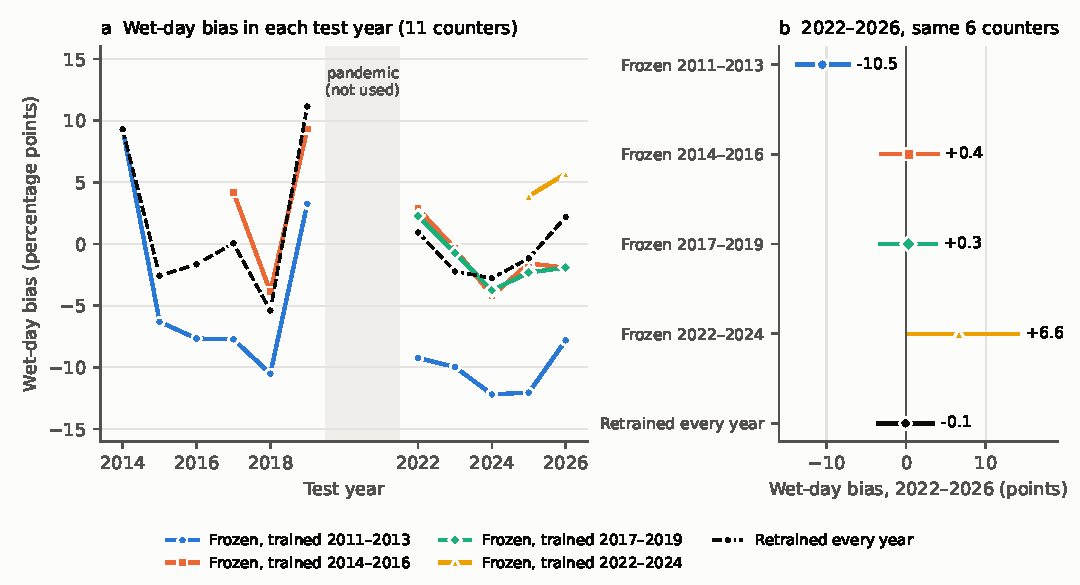
\includegraphics[width=\textwidth]{figures/fig_drift.pdf}
\caption{Wet-day bias of the forecasting models. (a) Each training strategy and test year, on the counters each model covers. (b) Test years 2022--2026 on the same six counters, with 95\% bootstrap intervals (check added after the results). Negative values: wet days are under-predicted compared with dry days in the same month at the same counter.}
\label{fig:drift}
\end{figure}

\subsection{The same counters (check added after the results)}

The model trained on 2011--2013 covers only six counters. To rule out that its bias comes from those counters, all models were compared on the same six counters (Figure~\ref{fig:drift}b). This check was not in the plan. On these counters, the wet-day bias in 2022--2026 was <<S_frozen_W1>> points (<<S_frozen_W1_ci>>) for the 2011--2013 model, against <<S_frozen_W2>> (<<S_frozen_W2_ci>>) for the 2014--2016 model and <<S_yearly>> (<<S_yearly_ci>>) for the retrained model. The difference between the 2011--2013 and 2014--2016 models was <<S_diffW2>> points (<<S_diffW2_ci>>). The bias is a property of the 2011--2013 model, not of its counters. On these counters the 2022--2024 model over-predicted wet days, with a wet-day bias of <<S_frozen_W4>> points (<<S_frozen_W4_ci>>).

\subsection{Overall accuracy}

Frozen models lost much of their accuracy over time, on dry days as well as on wet days (Table~\ref{tab:acc}). In 2022--2026 the frozen models had an error of <<accW3>> to <<accW1>> relative to last week's count, against <<accY>> for the retrained model. The model trained on 2011--2013 was barely better than the simple rule on dry days. The frozen model trained on 2022--2024 was slightly more accurate than yearly retraining in its two test years (<<accW4>> against <<accY2526>>), as one would expect from a model trained on the most recent years.

\begin{table}[!htbp]
\centering
\caption{Forecast error relative to the count on the same weekday a week earlier (1.0 = no better). All days, wet days and dry days.}
\label{tab:acc}
\footnotesize
\setlength{\tabcolsep}{4pt}
\begin{tabular}{@{}lcccccc@{}}
\toprule
 & \multicolumn{3}{c}{Test years 2014--2019} & \multicolumn{3}{c}{Test years 2022--2026} \\
\cmidrule(lr){2-4}\cmidrule(lr){5-7}
Training & All & Wet & Dry & All & Wet & Dry \\
\midrule
<<acc_rows>>
\bottomrule
\end{tabular}

\smallskip
\footnotesize $^{a}$ The model trained on 2022--2024 is tested only in 2025--2026. The retrained model on the same two years is shown for comparison.
\end{table}

\subsection{Neural networks}

The graph neural network (Graph WaveNet; \citealp{wu2019graph}) and the recurrent network of the earlier forecasting work were trained on recent years, from 2022 to April 2025. In the test period from June 2025 to November 2026, at 19 counters, they showed no wet-day under-prediction: <<E_gwn>> points for Graph WaveNet, <<E_rnn>> for the recurrent network and <<E_lgbm>> for LightGBM trained on all years. No frozen neural network was trained for this study.

\section{Discussion}

A forecasting model that is not retrained can go wrong on wet days when the way people respond to rain changes after it was trained. In Zurich this happened to the model trained on 2011--2013, which under-predicted wet days by about ten points a decade later. It did not happen to the models trained from 2014 onwards. What matters is therefore not the age of a model as such, but whether the weather response changed after its training data.

The forecasting models place the change earlier than the yearly rain effects of the companion study, which put most of it around 2017 \citep{arzimanli2026rain}. The two measure different things. The forecasting models learn the wet-day response given the counts of the previous days, while the companion study compares each day with dry days at the same counter in the same month. The check on the same counters rules out the choice of counters as the reason. It cannot rule out every difference between the early and later data, such as how the earliest counting devices behaved.

Frozen models also lost accuracy for reasons beyond the weather. Cycling grew strongly in these years, and travel patterns changed around the pandemic. The wet-day bias separates the part of the drift that comes from the weather response from this general loss. For practice, the results suggest two simple steps. Retrain at least once a year, which avoided both problems here. Add a wet-day check to the monitoring of a forecasting model: a regression of recent forecast errors on a wet-day indicator, within month and counter, shows whether the weather response is drifting even when the overall error looks acceptable. Methods for detecting drift and adapting to it \citep{alippi2013just,ditzler2015learning,gama2014survey} could be aimed at such condition-specific errors rather than at the overall error alone.

The study has limits. It covers one city, 11 counters and one type of model, and it uses the observed weather, which is the best case. The placebo test only just passed. The over-prediction of wet days by the model trained on 2022--2024 rests on two test years, and could be noise or the start of a further change. Graph models, which are increasingly used for traffic forecasting \citep{cini2025graph}, were only described here. Whether frozen graph models drift in the same way is an open question.

\section{Conclusion}

When the weather response of cyclists changes, a forecasting model that is not retrained can systematically under-predict wet days. In Zurich, a model trained on 2011--2013 did so by about ten points a decade later, while models trained from 2014 onwards and models retrained every year did not. Retraining every year and checking forecast errors on wet days separately are simple safeguards against this kind of drift.

\section*{Data and code availability}

All data are open. The code, the analysis plan with its checksums and the results are in the public repository \url{https://github.com/suadarzimanli/zurich-cycling-weather}, archived on Zenodo (\url{https://doi.org/10.5281/zenodo.24589808}). The plan for this study is \nolinkurl{docs/DRIFT_PLAN_2026-11-27.md}. The analysis is \nolinkurl{code/40_drift_forecast.py}, the check added after the results \nolinkurl{code/41_drift_check_counters.py}, and the figure \nolinkurl{code/42_drift_figure.py}.

\section*{Declaration of generative AI and AI-assisted technologies in the\\manuscript preparation process}

During the preparation of this work the author used Claude (Anthropic) to help design the study and its analysis plan, write and check the analysis code, produce the figure, search and verify the literature, and draft and revise the text, all under the author's direction. After using this tool, the author reviewed and edited the content as needed and takes full responsibility for the content of this paper.

\section*{Declaration of competing interest}

The author declares no known competing financial interests or personal relationships that could have appeared to influence the work reported in this paper.

\section*{Funding}

This research did not receive any specific grant from funding agencies in the public, commercial, or not-for-profit sectors.

\bibliographystyle{elsarticle-harv}
\bibliography{refs}

\end{document}
